\chapter{Formulario y pistas de la evaluación}
\label{Appendix:Key1}

En este anexo se recogen las capturas de pantalla asociadas al formulario completado por los usuarios. También se incluyen las pistas asociadas a cada tarea del formulario.

% TODO: \usepackage{graphicx} required
\begin{figure}[h!]
	\centering
	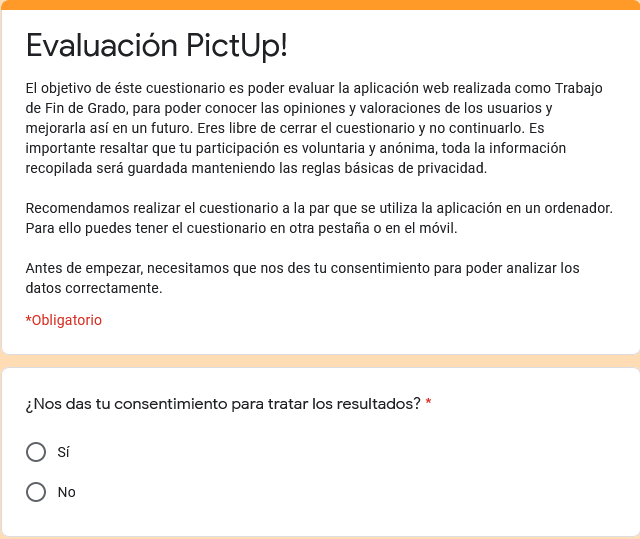
\includegraphics[width=0.7\linewidth]{Imagenes/Bitmap/formIntro}
	\caption{Introducción a la evaluación y consentimiento.}
	\label{fig:formintro}
\end{figure}

% TODO: \usepackage{graphicx} required
\begin{figure}[h!]
	\centering
	\includegraphics[width=0.7\linewidth]{Imagenes/Bitmap/formInformaciónPersonal}
	\caption{Preguntas de carácter demográfico.}
	\label{fig:forminformacionpersonal}
\end{figure}

% TODO: \usepackage{graphicx} required
\begin{figure}[h!]
	\centering
	\includegraphics[width=0.7\linewidth]{Imagenes/Bitmap/InformaciónPreviaAlForm}
	\caption{Introducción a las tareas y acceso a la aplicación.}
	\label{fig:informacionpreviaalform}
\end{figure}





% TODO: \usepackage{graphicx} required
\begin{figure}[h!]
	\centering
	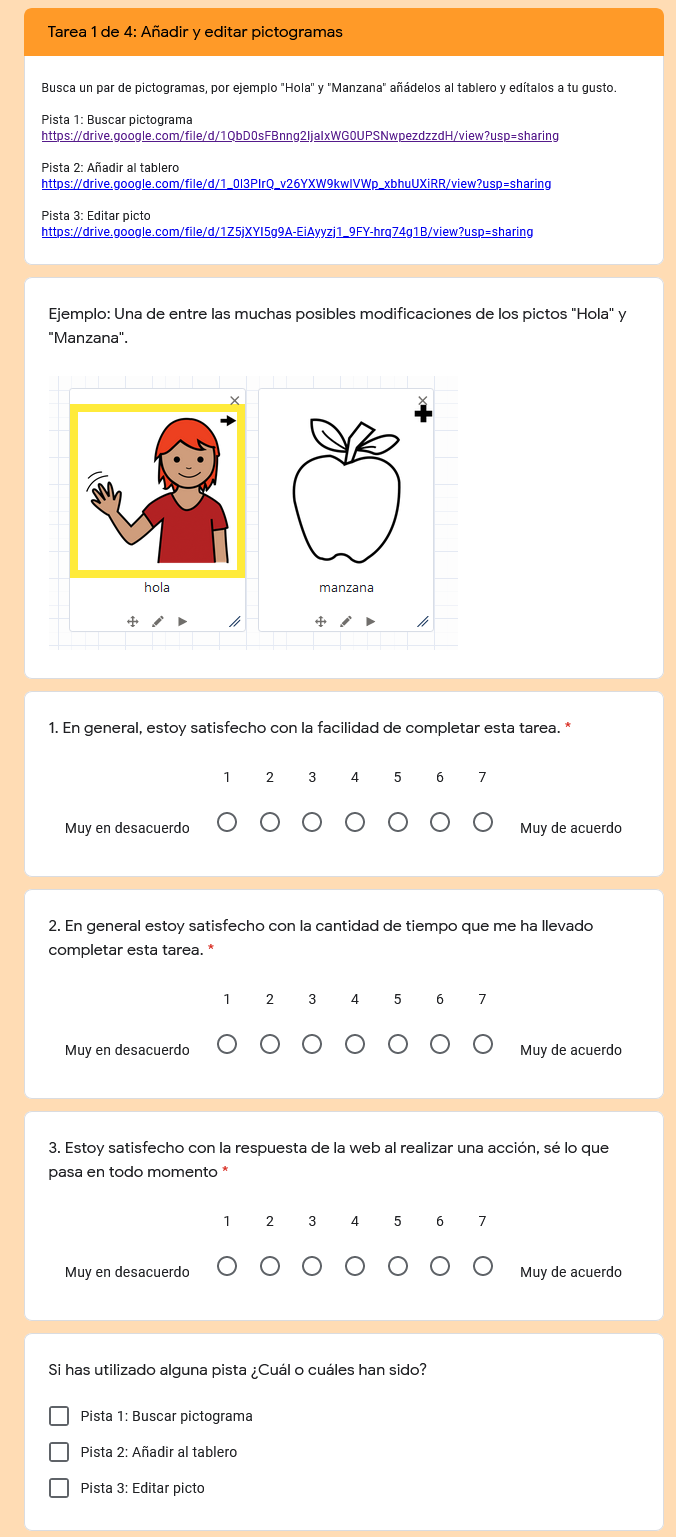
\includegraphics[width=0.78\linewidth]{Imagenes/Bitmap/Tarea1Preguntas}
	\caption{Descripción de la Tarea 1, pistas y preguntas.}
	\label{fig:tarea1preguntas}
\end{figure}


% TODO: \usepackage{graphicx} required
\begin{figure}[h!]
	\centering
	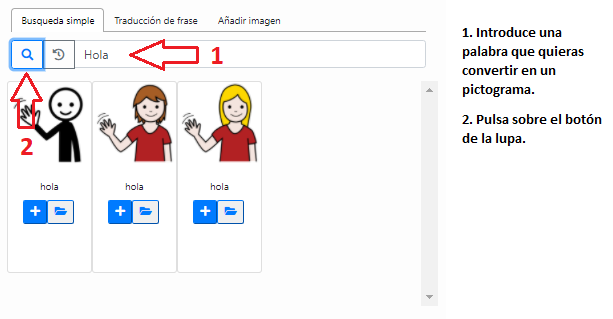
\includegraphics[width=0.7\linewidth]{Imagenes/Bitmap/Tarea1-Pista1}
	\caption{Buscar pictograma.}
	\label{fig:tarea1-pista1}
\end{figure}

% TODO: \usepackage{graphicx} required
\begin{figure}[h!]
	\centering
	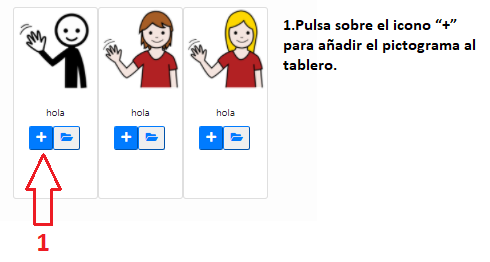
\includegraphics[width=0.7\linewidth]{Imagenes/Bitmap/Tarea1-Pista2}
	\caption{Añadir al tablero.}
	\label{fig:tarea1-pista2}
\end{figure}

% TODO: \usepackage{graphicx} required
\begin{figure}[h!]
	\centering
	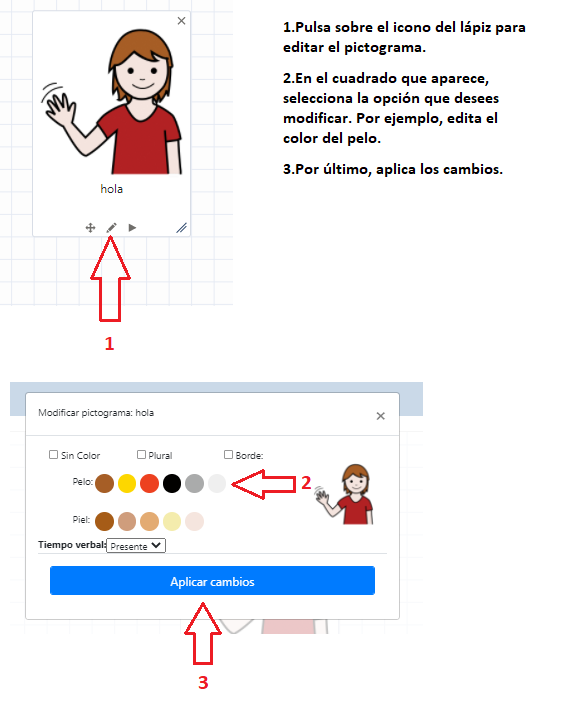
\includegraphics[width=0.7\linewidth]{Imagenes/Bitmap/Tarea1-Pista3}
	\caption{Editar picto.}
	\label{fig:tarea1-pista3}
\end{figure}



% TODO: \usepackage{graphicx} required
\begin{figure}[h!]
	\centering
	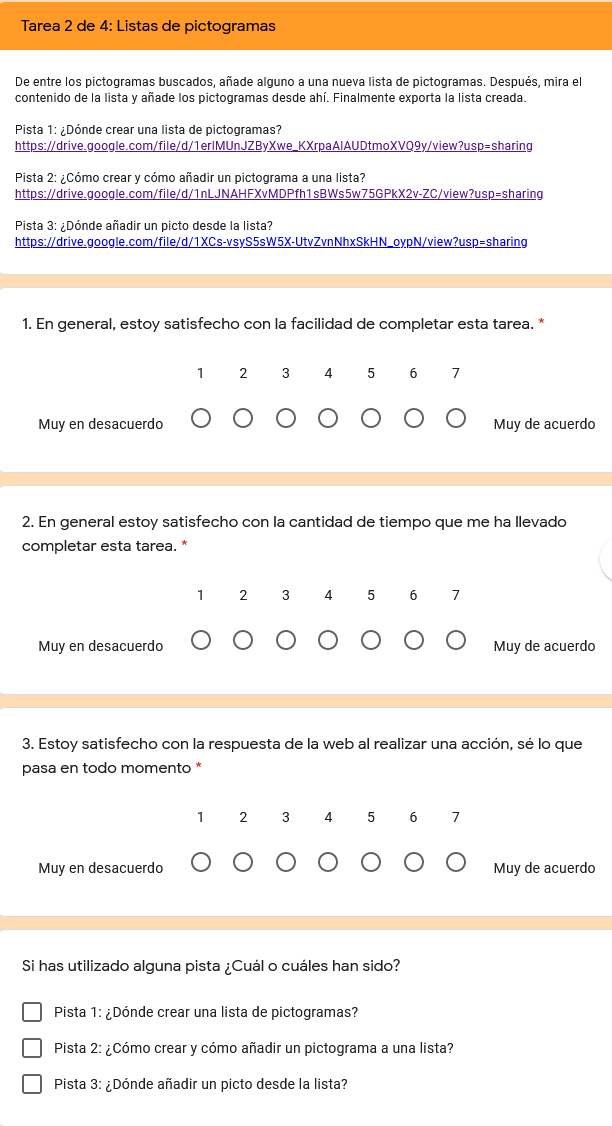
\includegraphics[width=0.78\linewidth]{Imagenes/Bitmap/Tarea2Preguntas}
	\caption{Descripción de la Tarea 2, pistas y preguntas.}
	\label{fig:tarea2preguntas}
\end{figure}

% TODO: \usepackage{graphicx} required
\begin{figure}[h!]
	\centering
	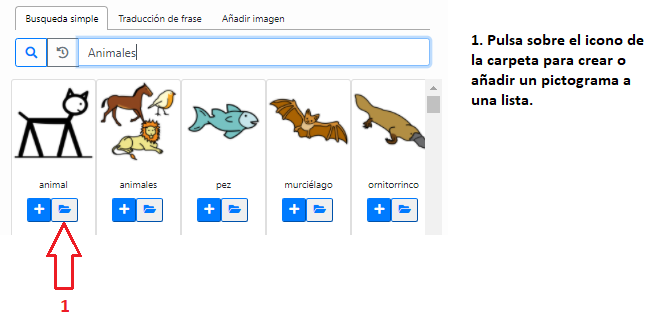
\includegraphics[width=0.7\linewidth]{Imagenes/Bitmap/Tarea2-Pista1}
	\caption{¿Dónde crear una lista de pictogramas?}
	\label{fig:tarea2-pista1}
\end{figure}

% TODO: \usepackage{graphicx} required
\begin{figure}[h!]
	\centering
	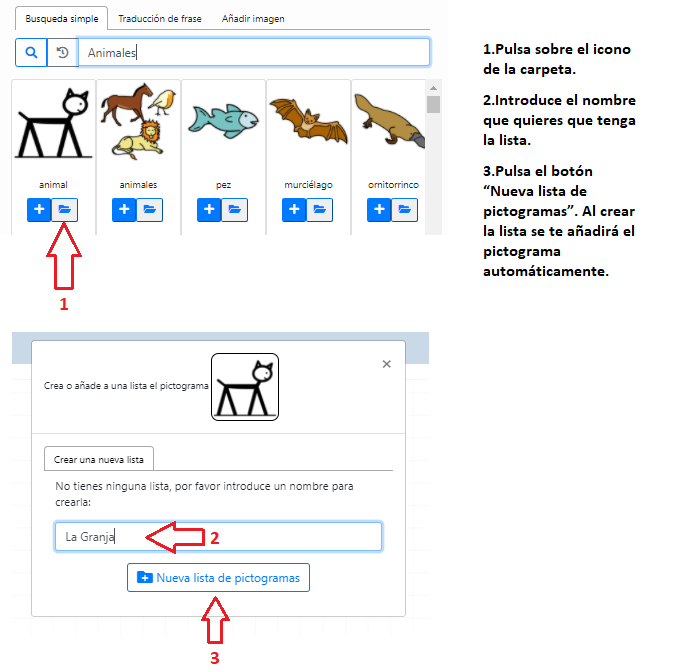
\includegraphics[width=0.7\linewidth]{Imagenes/Bitmap/Tarea2-Pista2}
	\caption{¿Cómo crear y cómo añadir un pictograma a una lista?}
	\label{fig:tarea2-pista2}
\end{figure}

% TODO: \usepackage{graphicx} required
\begin{figure}[h!]
	\centering
	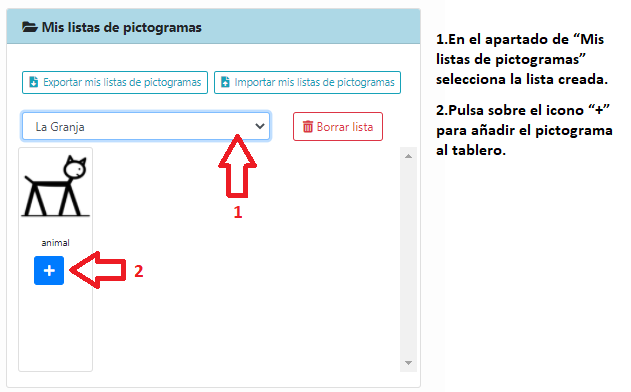
\includegraphics[width=0.7\linewidth]{Imagenes/Bitmap/Tarea2-Pista3}
	\caption{¿Dónde añadir un picto desde la lista?}
	\label{fig:tarea2-pista3}
\end{figure}


% TODO: \usepackage{graphicx} required
\begin{figure}[h!]
	\centering
	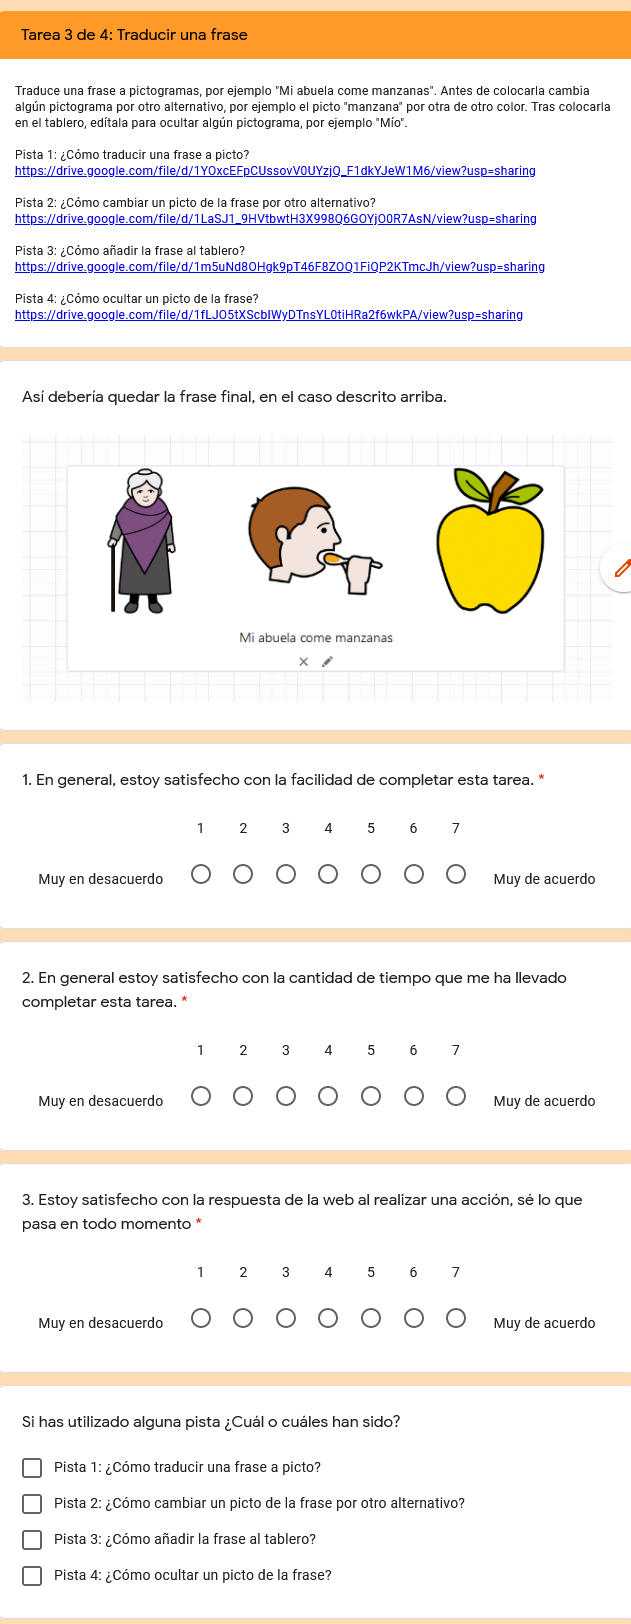
\includegraphics[width=0.6\linewidth]{Imagenes/Bitmap/Tarea3Preguntas}
	\caption{Descripción de la Tarea 3, pistas y preguntas.}
	\label{fig:tarea3preguntas}
\end{figure}

% TODO: \usepackage{graphicx} required
\begin{figure}[h!]
	\centering
	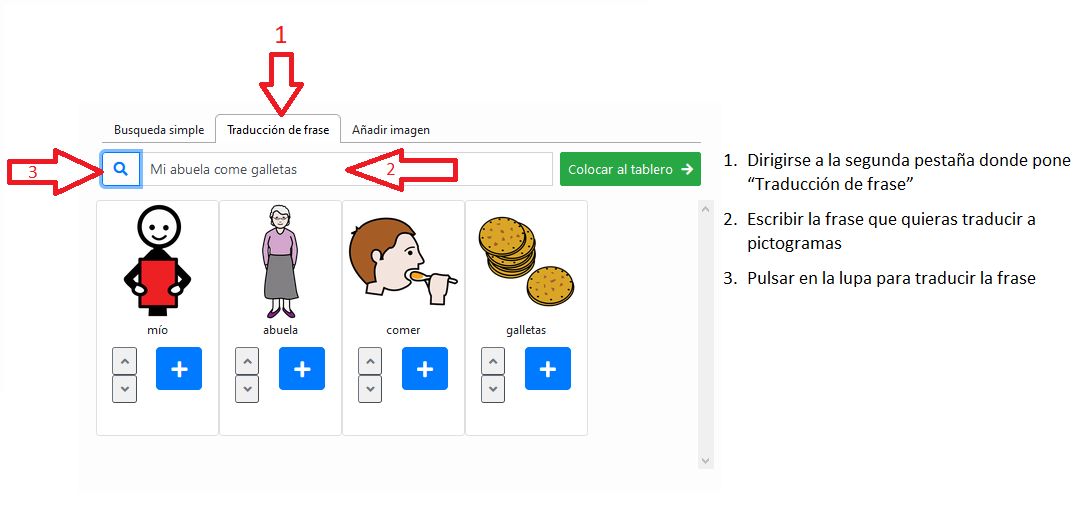
\includegraphics[width=0.7\linewidth]{Imagenes/Bitmap/Tarea3-Pista1}
	\caption{¿Cómo traducir una frase a picto?}
	\label{fig:tarea3-pista1}
\end{figure}


% TODO: \usepackage{graphicx} required
\begin{figure}[h!]
	\centering
	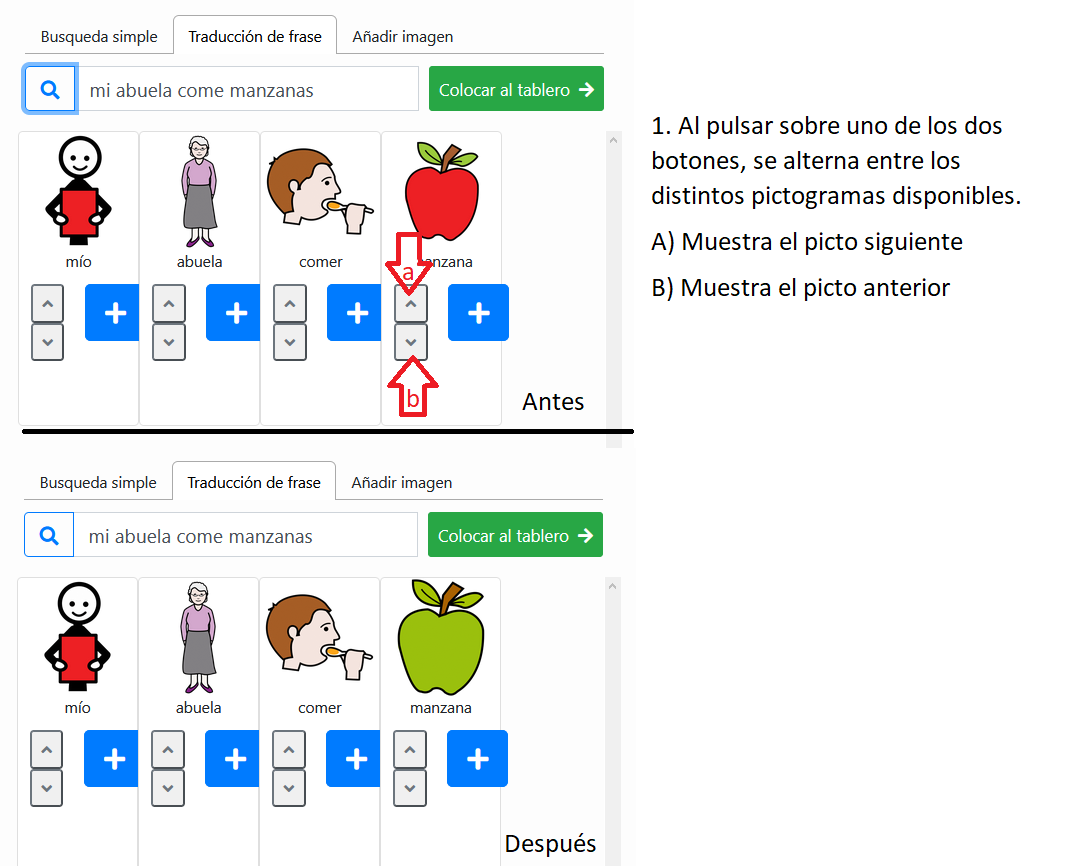
\includegraphics[width=0.7\linewidth]{Imagenes/Bitmap/Tarea3-Pista2}
	\caption{¿Cómo cambiar un picto de la frase por otro alternativo?}
	\label{fig:tarea3-pista2}
\end{figure}



% TODO: \usepackage{graphicx} required
\begin{figure}[h!]
	\centering
	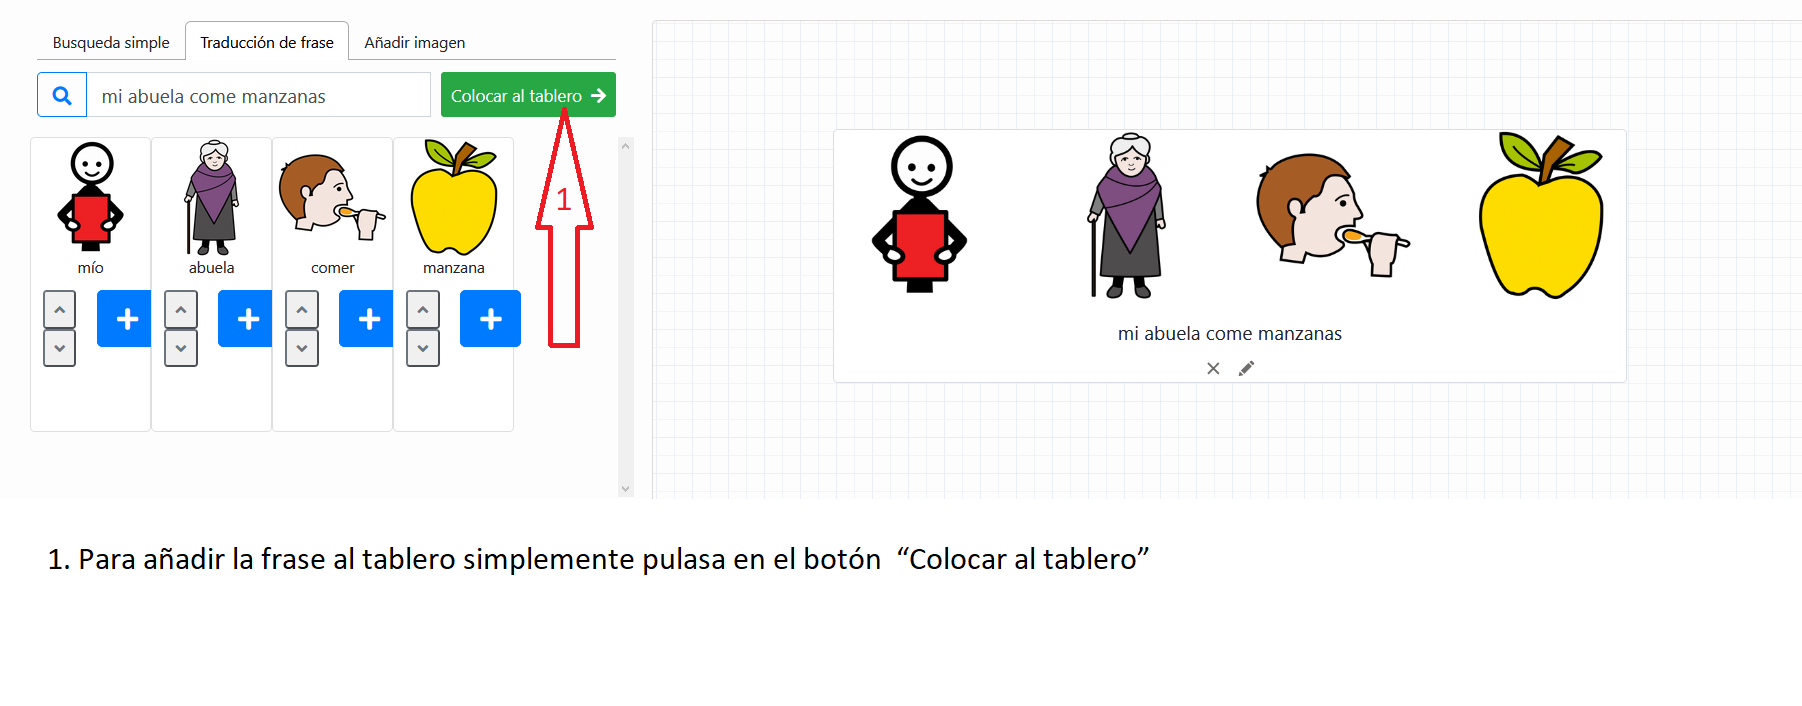
\includegraphics[width=0.7\linewidth]{Imagenes/Bitmap/Tarea3-Pista3}
	\caption{¿Cómo añadir la frase al tablero?}
	\label{fig:tarea3-pista3}
\end{figure}

% TODO: \usepackage{graphicx} required
\begin{figure}[h!]
	\centering
	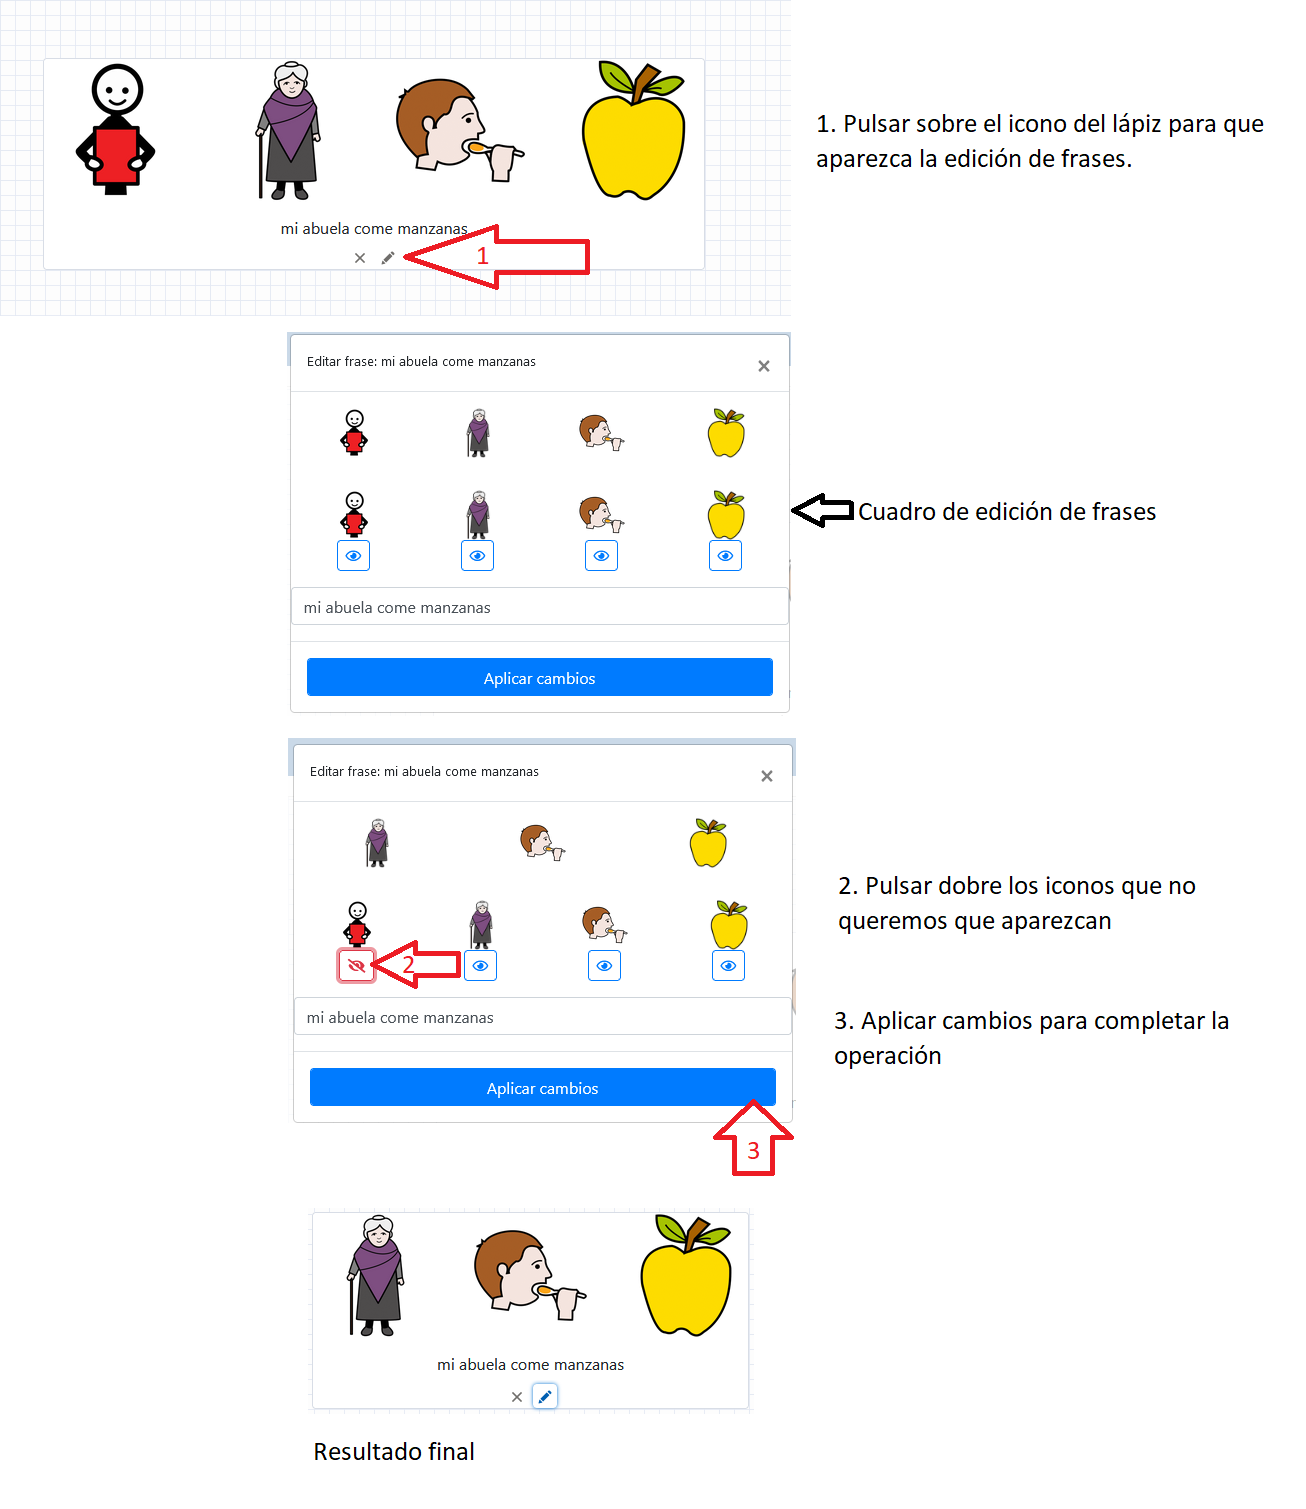
\includegraphics[width=0.7\linewidth]{Imagenes/Bitmap/Tarea3-Pista4}
	\caption{¿Cómo ocultar un picto de la frase?}
	\label{fig:tarea3-pista4}
\end{figure}


% TODO: \usepackage{graphicx} required
\begin{figure}[h!]
	\centering
	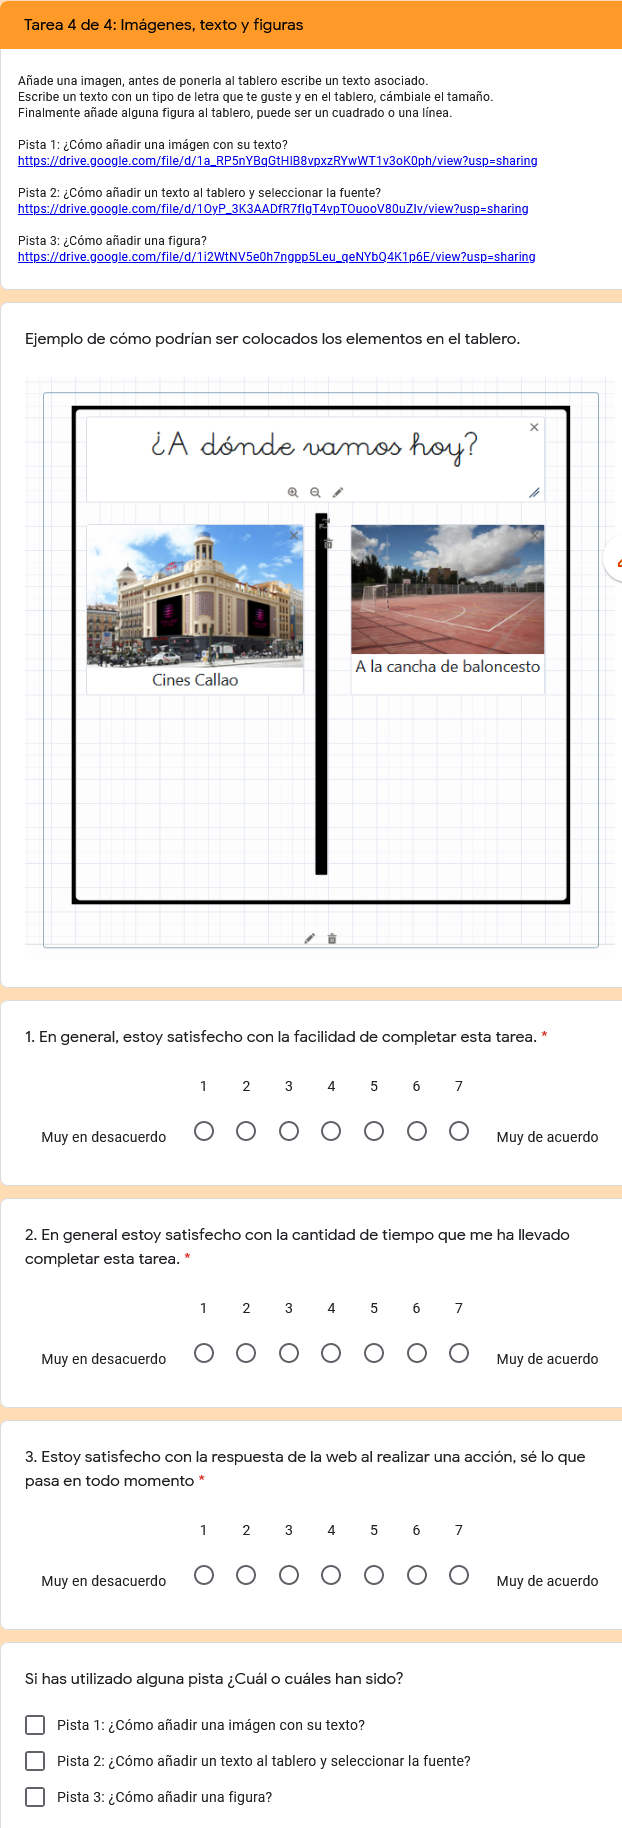
\includegraphics[width=0.6\linewidth]{Imagenes/Bitmap/Tarea4Preguntas}
	\caption{Descripción de la Tarea 4, pistas y preguntas.}
	\label{fig:tarea4preguntas}
\end{figure}


% TODO: \usepackage{graphicx} required
\begin{figure}[h!]
	\centering
	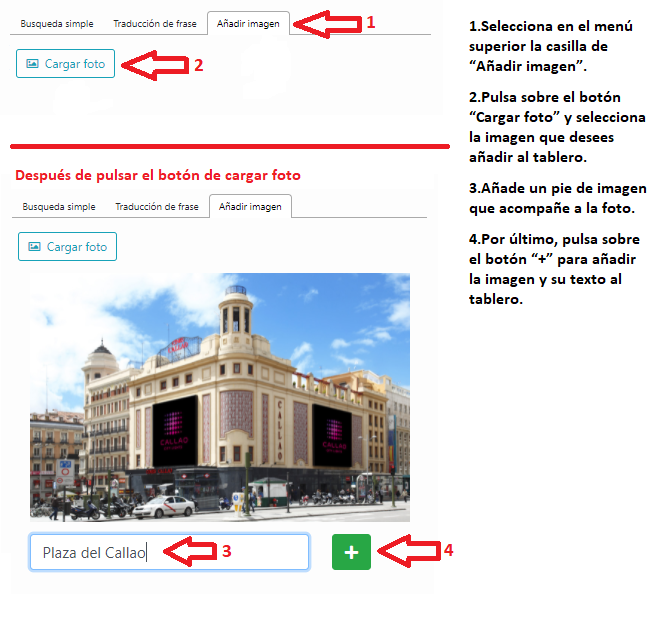
\includegraphics[width=0.7\linewidth]{Imagenes/Bitmap/Tarea4-Pista1}
	\caption{¿Cómo añadir una imágen con su texto?}
	\label{fig:tarea4-pista1}
\end{figure}

% TODO: \usepackage{graphicx} required
\begin{figure}[h!]
	\centering
	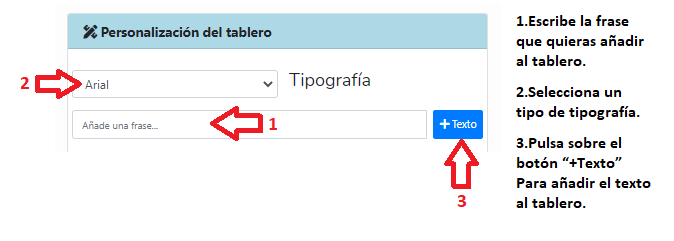
\includegraphics[width=0.7\linewidth]{Imagenes/Bitmap/Tarea4-Pista2}
	\caption{¿Cómo añadir un texto al tablero y seleccionar la fuente?}
	\label{fig:tarea4-pista2}
\end{figure}


% TODO: \usepackage{graphicx} required
\begin{figure}[h!]
	\centering
	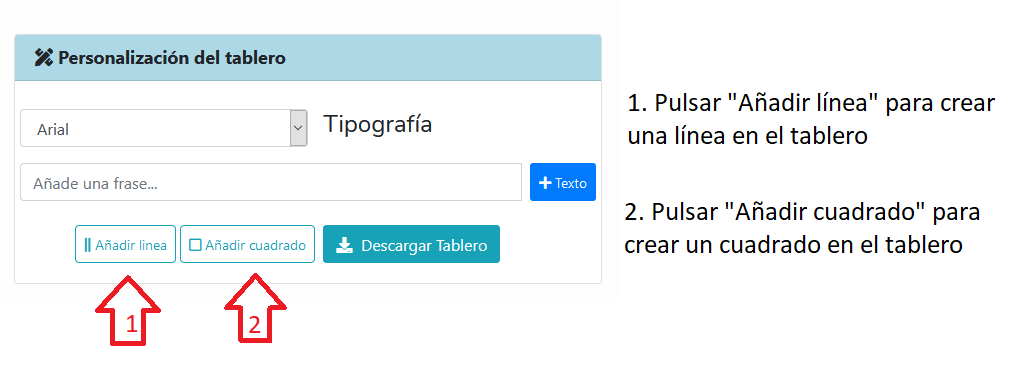
\includegraphics[width=0.7\linewidth]{Imagenes/Bitmap/Tarea4-Pista3}
	\caption{¿Cómo añadir una figura?}
	\label{fig:tarea4-pista3}
\end{figure}



% TODO: \usepackage{graphicx} required
\begin{figure}[h!]
	\centering
	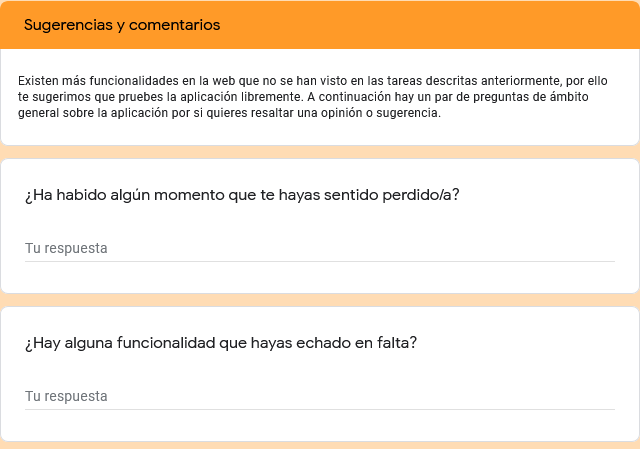
\includegraphics[width=0.7\linewidth]{Imagenes/Bitmap/Preguntas-respuestalibre}
	\caption{Pregunats de respuesta abierta.}
	\label{fig:preguntas-respuestalibre}
\end{figure}


% TODO: \usepackage{graphicx} required
\begin{figure}[h!]
	\centering
	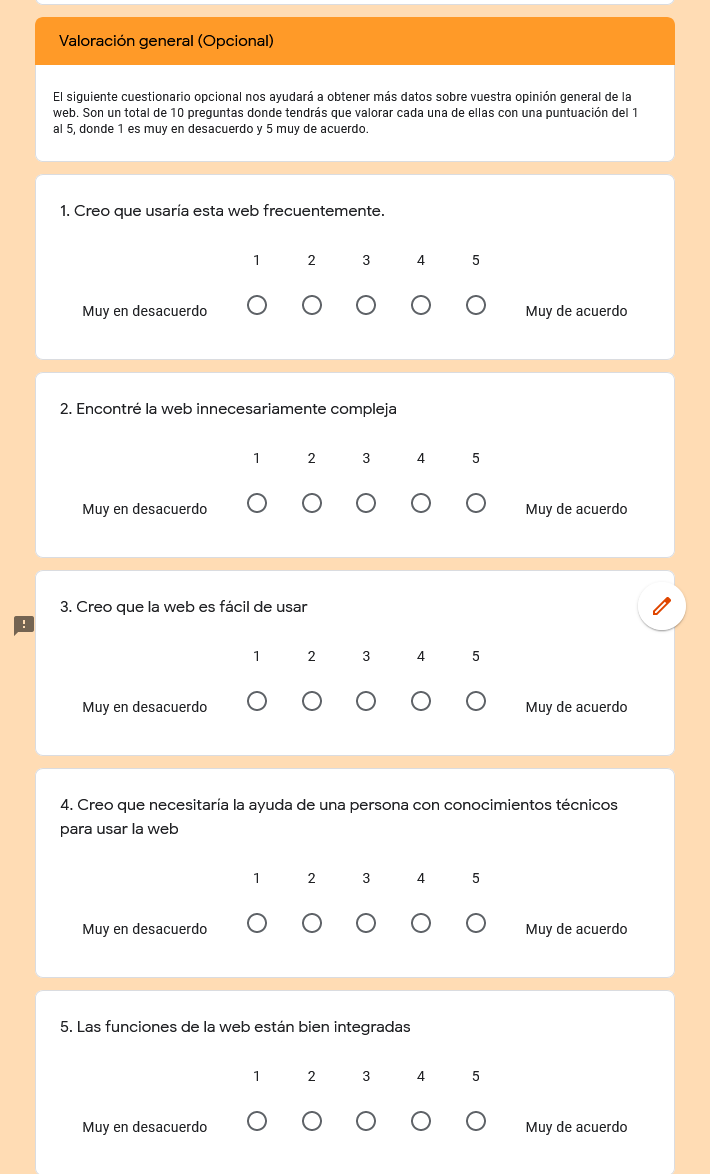
\includegraphics[width=0.7\linewidth]{Imagenes/Bitmap/Valoracion_general_sus1}
	\caption{Cuestionario SUS, preguntas 1-5.}
	\label{fig:valoraciongeneralsus1}
\end{figure}

% TODO: \usepackage{graphicx} required
\begin{figure}[h!]
	\centering
	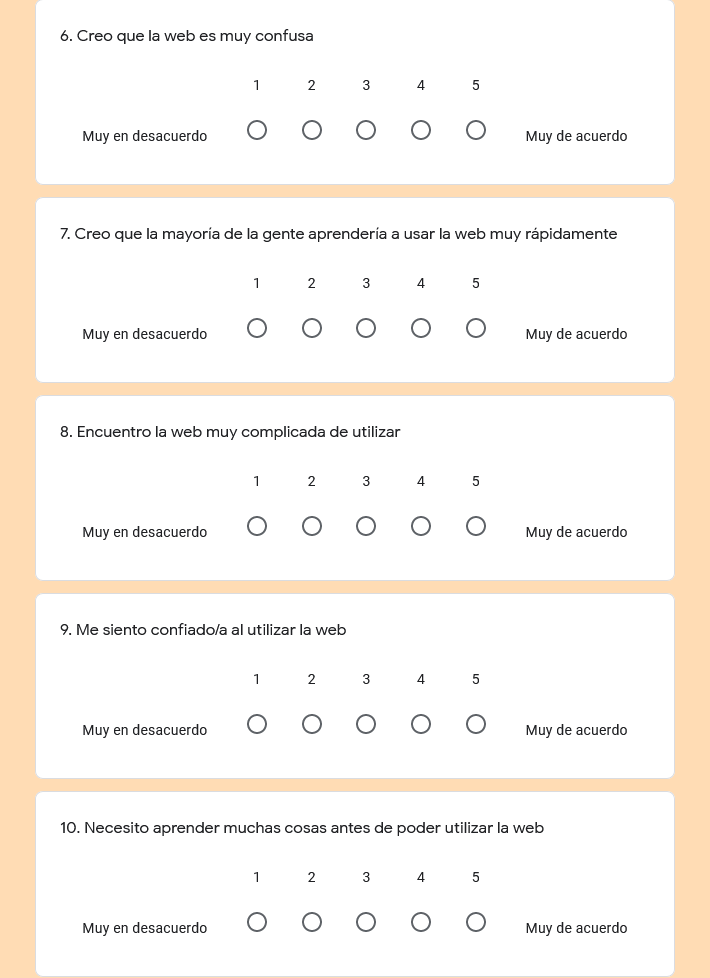
\includegraphics[width=0.7\linewidth]{Imagenes/Bitmap/Valoracion_general_sus2}
	\caption{Cuestionario SUS, preguntas 6-10.}
	\label{fig:valoraciongeneralsus2}
\end{figure}




